\section{Classifier}\label{sec:classifier}
As described in \cref{sec:machine_learning_task} we want to solve a supervised binary classification problem. In this section we will approach this problem by training a classifier based on training examples of article pairs. The feature extractor is used to extract features for these training examples, which are used to train a range of classifiers. Afterwards we evaluate the results and choose a classification algorithm for the system. Furthermore we describe how we optimize the classifier's parameters to increase performance.

\subsection{Training Data}\label{sec:training_data}
To train and evaluate a classifier we must first partition the positive and negative pairs $P$ and $N$, defined in \cref{sec:machine_learning_task}, into training and test data. To avoid overfitting on existing links, the training and testing data can not be used for feature learning. Therefore, we reserve a subset of $P$ that is only used for walks during feature learning.

We partition the positive training examples $P$ into three disjoint sets $P_\text{test}$, $P_\text{training}$, and $P_\text{walk}$ for testing, training, and feature learning walks, respectively. The partition is made randomly, with a distribution of 20\% test data, 40\% training data, and 40\% data for walks. This specific split is made to preserve the link structure in the graph while still having a reasonable amount of samples for testing and training.

%One sample of training data has the form \mono{<source article> <target article> <label>}. The source and targeet article are titles of pairs of articles. The label on the training samples can either be positive (link) or negative (do not link).

%Disjoint sets $P_{80} \subset P$ and $P_{20} \subset P$

As $\left\vert{P}\right\vert$ is smaller than $\left\vert{N}\right\vert$, we ensure an equal distribution of positive and negative training pairs, by randomly sampling two distinct sets $N_\text{test} \subset N$ and $N_\text{training} \subset N$, such that $\left\vert{N_\text{test}}\right\vert=\left\vert{P_\text{test}}\right\vert$ and $\left\vert{N_\text{training}}\right\vert=\left\vert{P_\text{training}}\right\vert$.

%The positive samples are pairs of articles $(a,b)$ such that article $a$ is featured and there exists a link from article $a$ to $b$.



%We first experimented with negative samples being random article pairs $(a,b)$ fulfilling the condition of $N$: that article $a$ is featured and there does not exist a link from article $a$ to $b$. The problem with this approach is that it is too easy to overfit using these negative samples. As the article pairs are randomly sampled, most of the times, there is very little relatedness between the two articles. This is of course the point of a negative training sample, but because most of the negative samples were so unrelated, the classifiers used in our experiments could too easily differentiate positives from negatives. We needed another method that would give us negative samples where the articles have a higher likelihood of being related. Our second approach was to extract N-grams from all featured articles. Iterating through all N-grams for a featured article, a negative sample would be generated if another article had the exact same title as the N-gram, but the two article were not linked.

\subsection{Choosing a Classifier}\label{choosing_classifier}
To get a coarse estimate of which classifier seems the most appropriate for our purpose, we create a test harness that will run a range of classification algorithms on the same dataset. This allows us to evaluate the performance of different classification algorithms. Each classifier is trained with default parameters, which might result in a suboptimal performance, but finding good parameters for all algorithms is unrealistic given the time frame of this project\todo{Kan vi undgå at nævne tiden?}\todo{Nogle har non-default for speed up}. Based on the results, we choose the algorithm that looks most promising to optimize further.

We examine a range of classifier available in the \emph{scikit-learn}~\cite{scikit-learn} Python library. This library provides a large selection of different classifiers, and as the classifiers share the same interface, it simplifies the test harness.

\subsubsection{Evaluation Metrics}\label{evaluation_metric}
To evaluate the performance of each algorithm, we perform a 10-fold cross-validation. As the core of our problem definition is to produce reasonable suggestions of missing links, false positives should be punished harder than false negatives. A false positive is an incorrect classification of a negative example, where a false negative is an incorrect classification of a positive example. Essentially, we believe it is worse to falsely suggest a pair of articles to be linked, than not suggest a pair of articles that should be linked.

Because of the before mentioned higher penalty rate of false positives we want to favor precision over recall, as precision decreases as the number of false positives increases.

A common measure of a test's accuracy is the \emph{F-score}, which considers both precision and recall. Variants exists that weighs precision higher than recall, but because we want to minimize the amount of false positives we consider precision as our primary evaluation metric.

\begin{equation}\label{eq:precision}
\text{Precision} = \frac{\text{true positives}}{\text{true positives} + \text{false positives}}
\end{equation}

\begin{equation}\label{eq:recall}
\text{Recall} = \frac{\text{true positives}}{\text{true positives} + \text{false negatives}}
\end{equation}


\subsubsection{Results}
A bar chart of results can be seen in \cref{fig:classifier_comparison}. \emph{QDA} gives the best precision of $0.985$. However the recall is low, which is a cause for concern, as this implies a reduced number of suggestions. The second highest precision, \emph{Nearest Centroid}, gives a precision of $0.979$ which is slightly lower than \emph{QDA}, but with a far better recall. Though we consider precision the most important metric, trading $0.6\%$ precision for much better recall seems favorable, and we therefore use the \emph{Nearest Centroid} classifier. The \emph{nearest centroid} classifier has no parameters, avoiding the optimization process.

%\begin{figure}[tbp]
%\centering
%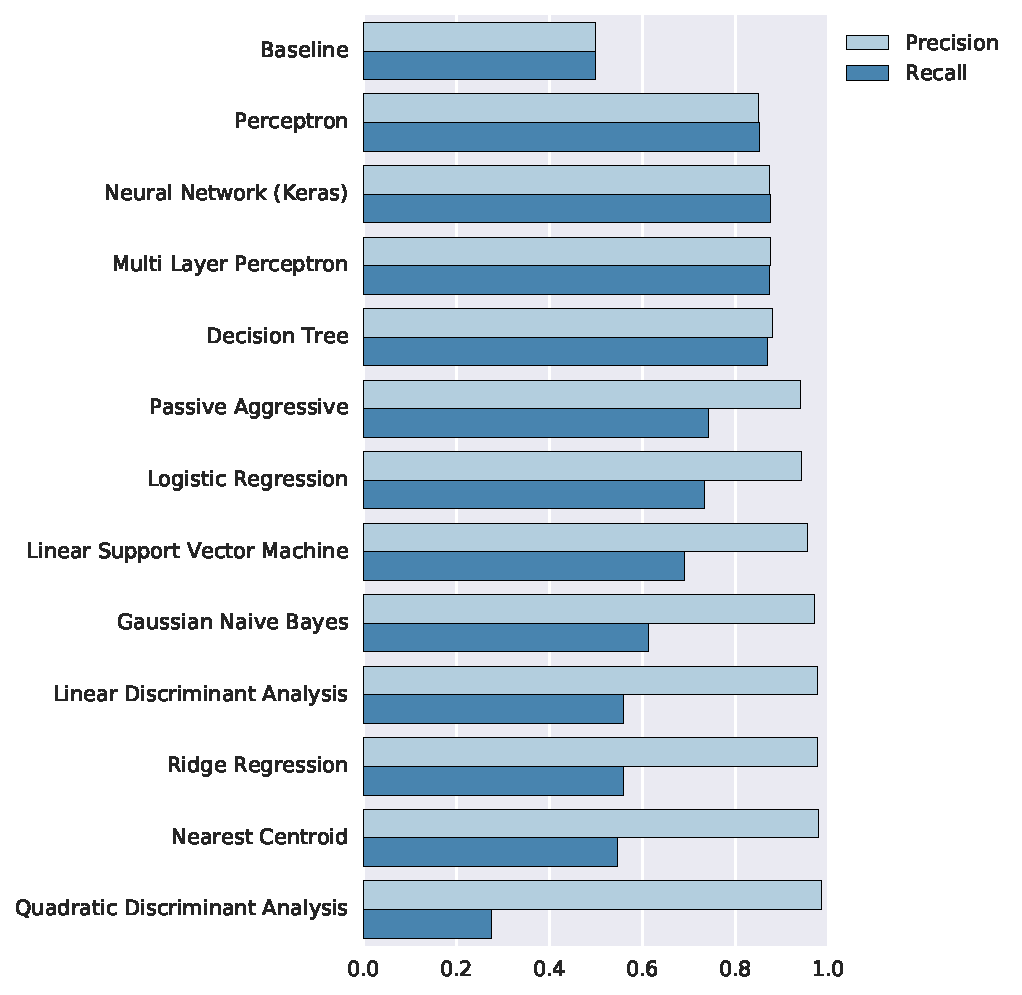
\includegraphics[width=0.95\textwidth]{classifier-comparison2.pdf}
%\caption[Precision and recall scores for the chosen algorithms]{Precision and recall scores for the chosen algorithms, sorted by precision.}\label{fig:classifier_comparison}
%\end{figure}

\begin{figure}%
\centering
\tikzsetnextfilename{barchart}
\begin{tikzpicture}
  \begin{axis}[
      table/col sep=semicolon,
      xbar=0pt, xmin=0, xmax=1,
      xlabel=Score,
      yticklabels from table={chapter_design/precision.csv}{name},
      %yticklabel style={text height=1.5ex},
      ytick=data,
      width=0.6\textwidth,
      y=0.9cm,
      enlarge y limits={abs=0.6},
      bar width=8pt,
      /pgf/number format/fixed,
      axis lines*=left,
      xmajorgrids=true,
      legend entries={Recall, Precision},
      legend style={draw=none},
      reverse legend, area legend,
      legend style={at={(1,1.01)},anchor=south east}
    ]
    \addplot [fill=color1!20!white] table [y expr=-\coordindex, x=recall] {chapter_design/precision.csv};
    \addplot [fill=color1!70!white] table [y expr=-\coordindex, x=precision] {chapter_design/precision.csv};

  \end{axis}
\end{tikzpicture}
\caption[Precision and recall scores for the chosen algorithms]{Precision and recall scores for the chosen algorithms, sorted by precision}\label{fig:classifier_comparison}%
\end{figure}

% \begin{table}[tbp]
% \centering
% \begin{tabular}{@{}lp{.75\textwidth}@{}}
% \toprule
% \textbf{Classifier} & \textbf{Result} \\
% \midrule
% Baseline           &  DummyClassifier()                \\
% Nearest Neighbors  &  KNeighborsClassifier(3)          \\
% Linear SVM         &  SVC(kernel="linear", C=0.025)    \\
% RBF SVM            &  SVC(gamma=2, C=1)                \\
% Gaussian Process   &  GaussianProcessClassifier        \\
% Decision Tree      &  DecisionTreeClassifier           \\
% Random Forest      &  RandomForestClassifier           \\
% Neural Net         &  MLPClassifier, KerasClassifier   \\
% AdaBoost           &  AdaBoostClassifier()             \\
% Naive Bayes        &  GaussianNB()                     \\
% QDA                &  QuadraticDiscriminantAnalysis()  \\
% \bottomrule
% \end{tabular}
% \caption[Classifiers]{Classifiers}%
% \label{tab:classifiers}
% \end{table}

% \subsection{Classifier Parameter Optimization}
% To attempt to further increase the performance of the chosen classifier, we optimize its parameters. The \emph{nearest centroid} implementation in the \emph{scikit-learn} library only has two parameters, so we use grid search to explore possible parameter combinations, as the parameter space is small.

% Searching the parameter space reveals that the default parameters, with a euclidean distance metric, and no feature shrink threshold specified, gives the best performance.
